\documentclass[10pt]{article}
\usepackage[polish]{babel}
\usepackage[utf8]{inputenc}
\usepackage[T1]{fontenc}
\usepackage{amsmath}
\usepackage{amsfonts}
\usepackage{amssymb}
\usepackage[version=4]{mhchem}
\usepackage{stmaryrd}
\usepackage{graphicx}
\usepackage[export]{adjustbox}
\graphicspath{ {./images/} }

\title{PRÓBNY EGZAMIN MATURALNY Z MATEMATYKI }

\author{}
\date{}


\begin{document}
\maketitle
Arkusz zawiera informacje prawnie chronione do momentu rozpoczęcia egzaminu.\\
WPISUJE ZDAJĄCY\\
KOD

\begin{center}
\begin{tabular}{|l|l|l|l|l|l|l|l|l|l|}
 &  &  &  &  &  &  &  &  \\
\hline
 &  &  &  &  &  &  &  &  \\
\hline
 &  &  &  &  &  &  &  &  \\
Miejsce &  &  &  &  &  &  &  &  \\
na naklejke &  &  &  &  &  &  &  &  \\
\(z\) kodem &  &  &  &  &  &  &  &  \\
\end{tabular}
\end{center}

\section*{POZIOM PODSTAWOWY}
\begin{enumerate}
  \item Sprawdź, czy arkusz egzaminacyjny zawiera 19 stron (zadania 1-34). Ewentualny brak zgłoś przewodniczącemu zespołu nadzorującego egzamin.
  \item Rozwiazania zadań i odpowiedzi wpisuj w miejscu na to przeznaczonym.
  \item Odpowiedzi do zadań zamkniętych (1-25) przenieś na kartę odpowiedzi, zaznaczając je w części karty przeznaczonej dla zdającego. Zamaluj ■ pola do tego przeznaczone. Błędne zaznaczenie otocz kółkiem i zaznacz właściwe.
  \item Pamiętaj, że pominięcie argumentacji lub istotnych obliczeń w rozwiązaniu zadania otwartego (26-34) może spowodować, że za to rozwiązanie nie będziesz mógł dostać pełnej liczby punktów.
  \item Pisz czytelnie i używaj tylko długopisu lub pióra z czarnym tuszem lub atramentem.
  \item Nie używaj korektora, a błędne zapisy wyraźnie przekreśl.
  \item Pamiętaj, że zapisy w brudnopisie nie będą oceniane.
  \item Możesz korzystać z zestawu wzorów matematycznych, cyrkla i linijki oraz kalkulatora.
  \item Na karcie odpowiedzi wpisz i zakoduj swój numer PESEL.
  \item Nie wpisuj żadnych znaków w części przeznaczonej dla egzaminatora.
\end{enumerate}

Liczba punktów do uzyskania: 50

Czas pracy: 170 minut\\

\includegraphics[max width=\textwidth, center]{2024_11_21_603d5c1b2a7d8d68f45fg-01}

MMA-P1\_1P-105

\section*{ZADANIA ZAMKNIĘTE}
\section*{W zadaniach od 1. do 25. wybierz i zaznacz na karcie odpowiedzi jedna}
poprawnq odpowiedź.

\section*{Zadanie 1. (1 pkt)}
Liczba \(|5-7|-|-3+4|\) jest równa\\
A. -3\\
B. -5\\
C. 1\\
D. 3

\section*{Zadanie 2. (1 pkt)}
Wskaż rysunek, na którym jest przedstawiony zbiór rozwiązań nierówności \(|x-2| \geq 3\).\\
A.\\
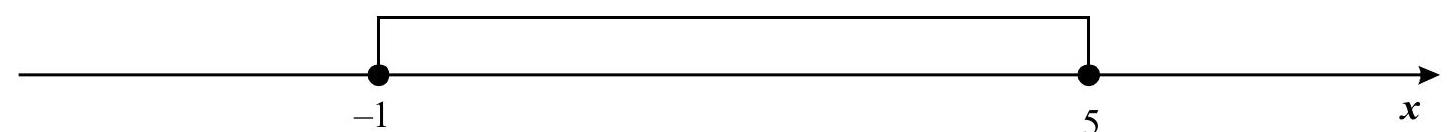
\includegraphics[max width=\textwidth, center]{2024_11_21_603d5c1b2a7d8d68f45fg-02(2)}\\
B.\\
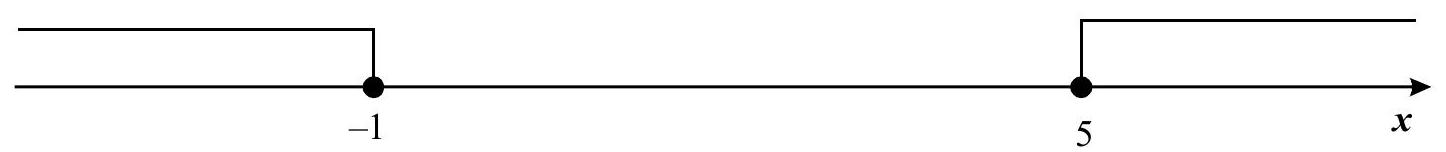
\includegraphics[max width=\textwidth, center]{2024_11_21_603d5c1b2a7d8d68f45fg-02}\\
C.\\
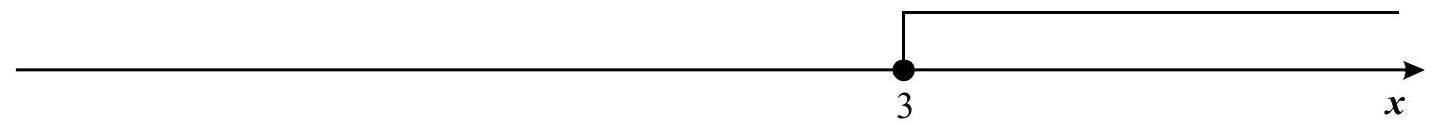
\includegraphics[max width=\textwidth, center]{2024_11_21_603d5c1b2a7d8d68f45fg-02(1)}\\
D.\\
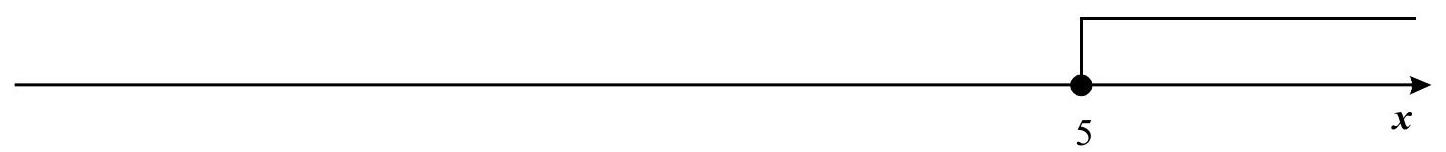
\includegraphics[max width=\textwidth, center]{2024_11_21_603d5c1b2a7d8d68f45fg-02(3)}

\section*{Zadanie 3. (1 pkt)}
Samochód kosztował 30000 zł. Jego cenę obniżono o \(10 \%\), a następnie cenę po tej obniżce ponownie obniżono o \(10 \%\). Po tych obniżkach samochód kosztował\\
A. 24400 zt\\
B. 24700 zt\\
C. 24000 zl\\
D. 24300 zt

\section*{Zadanie 4. (1 pkt)}
Dana jest liczba \(x=63^{2} \cdot\left(\frac{1}{3}\right)^{4}\). Wtedy\\
A. \(x=7^{2}\)\\
B. \(x=7^{-2}\)\\
C. \(x=3^{8} \cdot 7^{2}\)\\
D. \(x=3 \cdot 7\)

\section*{Zadanie 5. (1 pkt)}
Kwadrat liczby \(x=5+2 \sqrt{3}\) jest równy\\
A. 37\\
B. \(25+4 \sqrt{3}\)\\
C. \(37+20 \sqrt{3}\)\\
D. 147

\section*{Zadanie 6. (1 pkt)}
Liczba \(\log _{5} 5-\log _{5} 125\) jest równa\\
A. -2\\
B. -1\\
C. \(\frac{1}{25}\)\\
D. 4\\

\includegraphics[max width=\textwidth, center]{2024_11_21_603d5c1b2a7d8d68f45fg-03}

W zadaniach 7, 8 i 9 wykorzystaj przedstawiony poniz̈ej wykres funkcji \(f\).\\
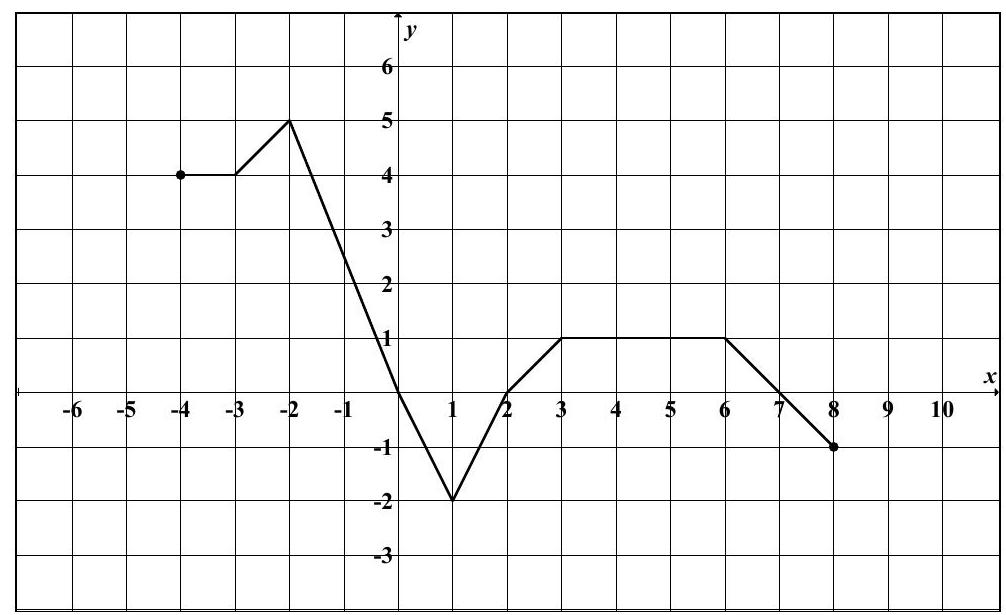
\includegraphics[max width=\textwidth, center]{2024_11_21_603d5c1b2a7d8d68f45fg-04(4)}

\section*{Zadanie 7. (1 pkt)}
Zbiorem wartości funkcji \(f\) jest\\
A. \(\langle-2,5\rangle\)\\
B. \(\langle-4,8\rangle\)\\
C. \(\langle-1,4\rangle\)\\
D. \(\langle 5,8\rangle\)

\section*{Zadanie 8. (1 pkt)}
Korzystając z wykresu funkcji \(f\), wskaż nierówność prawdziwą.\\
A. \(f(-1)<f(1)\)\\
B. \(f(1)<f(3)\)\\
C. \(f(-1)<f(3)\)\\
D. \(f(3)<f(0)\)

\section*{Zadanie 9. (1 pkt)}
Wykres funkcji \(g\) określonej wzorem \(g(x)=f(x)+2\) jest przedstawiony na rysunku\\
A.\\
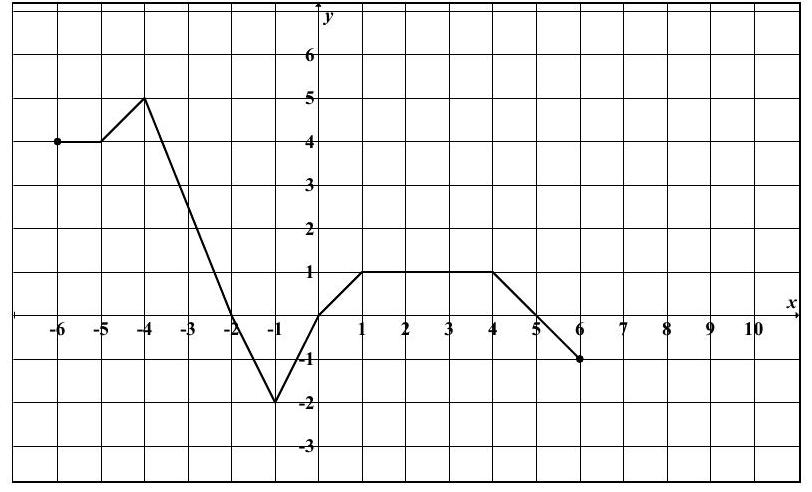
\includegraphics[max width=\textwidth, center]{2024_11_21_603d5c1b2a7d8d68f45fg-04(2)}\\
C.\\
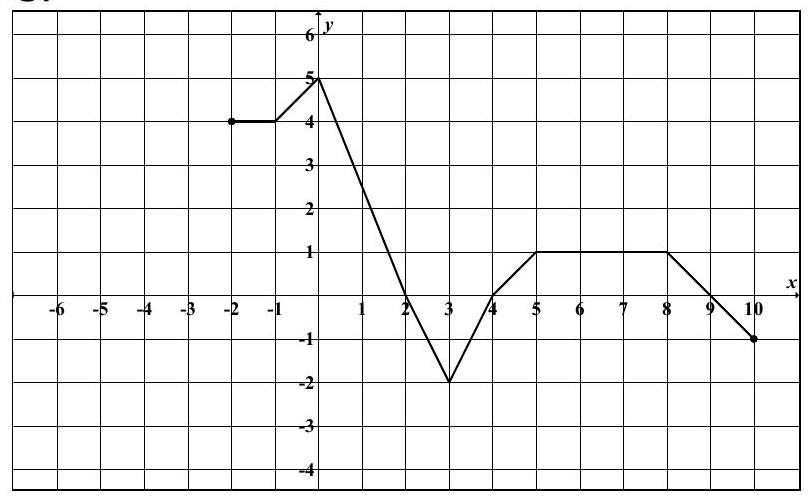
\includegraphics[max width=\textwidth, center]{2024_11_21_603d5c1b2a7d8d68f45fg-04}\\
B.\\
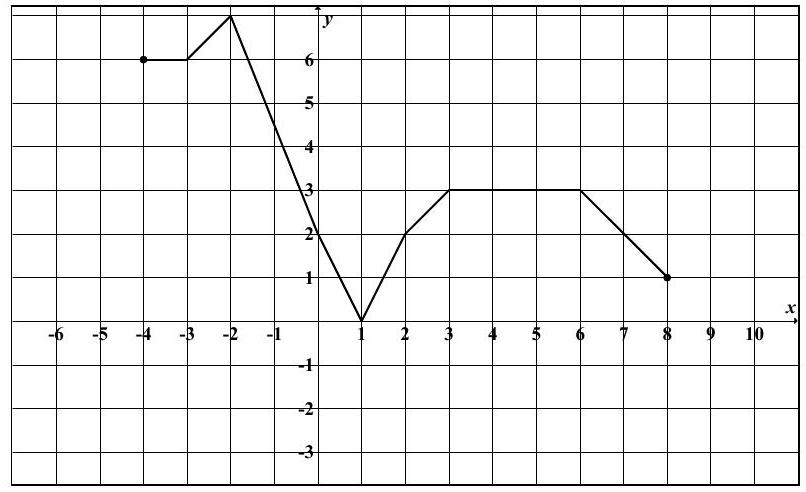
\includegraphics[max width=\textwidth, center]{2024_11_21_603d5c1b2a7d8d68f45fg-04(3)}\\
D.\\
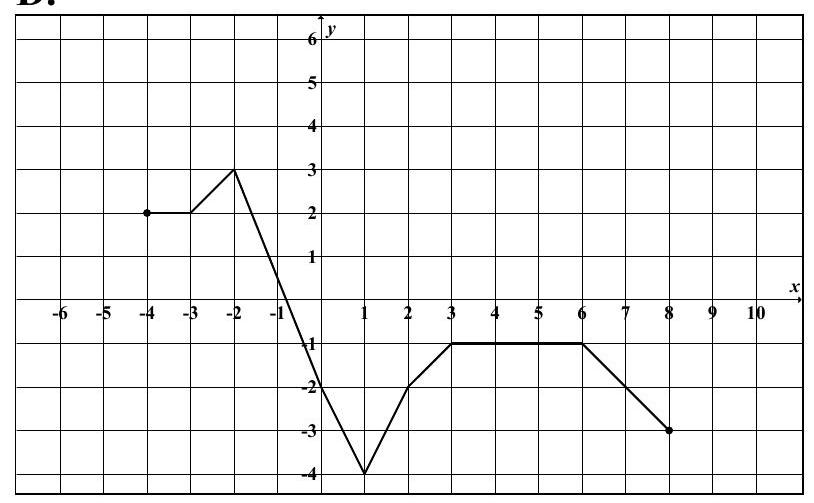
\includegraphics[max width=\textwidth, center]{2024_11_21_603d5c1b2a7d8d68f45fg-04(1)}\\

\includegraphics[max width=\textwidth, center]{2024_11_21_603d5c1b2a7d8d68f45fg-05}

\section*{Zadanie 10. (1 pkt)}
Liczby \(x_{1}\) i \(x_{2}\) są pierwiastkami równania \(x^{2}+10 x-24=0\) i \(x_{1}<x_{2}\). Oblicz \(2 x_{1}+x_{2}\).\\
A. -22\\
B. -17\\
C. 8\\
D. 13

\section*{Zadanie 11. (1 pkt)}
Liczba 2 jest pierwiastkiem wielomianu \(W(x)=x^{3}+a x^{2}+6 x-4\). Współczynnik \(a\) jest równy\\
A. 2\\
B. -2\\
C. 4\\
D. -4

\section*{Zadanie 12. (1 pkt)}
Wskaż \(m\), dla którego funkcja liniowa określona wzorem \(f(x)=(m-1) x+3\) jest stała.\\
A. \(m=1\)\\
B. \(m=2\)\\
C. \(m=3\)\\
D. \(m=-1\)

\section*{Zadanie 13. (1 pkt)}
Zbiorem rozwiązań nierówności \((x-2)(x+3) \geq 0\) jest\\
A. \(\langle-2,3\rangle\)\\
B. \(\langle-3,2\rangle\)\\
C. \((-\infty,-3\rangle \cup\langle 2,+\infty)\)\\
D. \((-\infty,-2\rangle \cup\langle 3,+\infty)\)

\section*{Zadanie 14. (1 pkt)}
W ciagu geometrycznym \(\left(a_{n}\right)\) dane sa: \(a_{1}=2\) i \(a_{2}=12\). Wtedy\\
A. \(a_{4}=26\)\\
B. \(a_{4}=432\)\\
C. \(a_{4}=32\)\\
D. \(a_{4}=2592\)

\section*{Zadanie 15. (1 pkt)}
W ciagu arytmetycznym \(a_{1}=3\) oraz \(a_{20}=7\). Wtedy suma \(S_{20}=a_{1}+a_{2}+\ldots+a_{19}+a_{20}\) jest równa\\
A. 95\\
B. 200\\
C. 230\\
D. 100

\section*{Zadanie 16. (1 pkt)}
Na rysunku zaznaczono długości boków i kąt \(\alpha\) trójkąta prostokątnego (zobacz rysunek). Wtedy\\
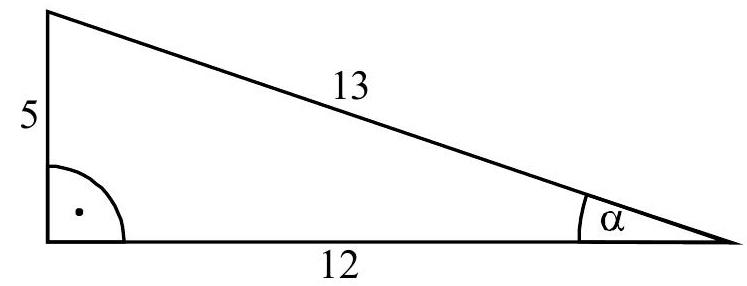
\includegraphics[max width=\textwidth, center]{2024_11_21_603d5c1b2a7d8d68f45fg-06}\\
A. \(\cos \alpha=\frac{5}{13}\)\\
B. \(\operatorname{tg} \alpha=\frac{13}{12}\)\\
C. \(\cos \alpha=\frac{12}{13}\)\\
D. \(\operatorname{tg} \alpha=\frac{12}{5}\)\\

\includegraphics[max width=\textwidth, center]{2024_11_21_603d5c1b2a7d8d68f45fg-07}

\section*{Zadanie 17. (1 pkt)}
Ogród ma kształt prostokąta o bokach długości 20 m i 40 m . Na dwóch końcach przekątnej tego prostokąta wbito słupki. Odległość między tymi słupkami jest\\
A. równa 40 m\\
B. większa niż 50 m\\
C. większa niż 40 m i mniejsza niż 45 m\\
D. większa niż 45 m i mniejsza niż 50 m

\section*{Zadanie 18. (1 pkt)}
Pionowy słupek o wysokości 90 cm rzuca cień o długości 60 cm . W tej samej chwili stojąca obok wieża rzuca cień długości 12 m . Jaka jest wysokość wieży?\\
A. 18 m\\
B. 8 m\\
C. 9 m\\
D. 16 m

\section*{Zadanie 19. (1 pkt)}
Punkty \(A, B\) i \(C\) leżą na okręgu o środku \(S\) (zobacz rysunek). Miara zaznaczonego kąta wpisanego \(A C B\) jest równa\\
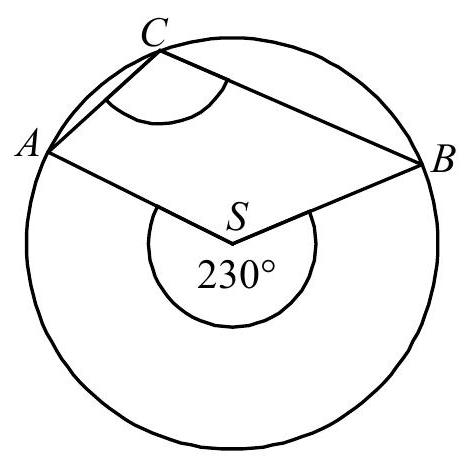
\includegraphics[max width=\textwidth, center]{2024_11_21_603d5c1b2a7d8d68f45fg-08}\\
A. \(65^{\circ}\)\\
B. \(100^{\circ}\)\\
C. \(115^{\circ}\)\\
D. \(130^{\circ}\)

\section*{Zadanie 20. (1 pkt)}
Dane są punkty \(S=(2,1), M=(6,4)\). Równanie okręgu o środku \(S\) i przechodzacego przez punkt \(M\) ma postać\\
A. \((x-2)^{2}+(y-1)^{2}=5\)\\
B. \((x-2)^{2}+(y-1)^{2}=25\)\\
C. \((x-6)^{2}+(y-4)^{2}=5\)\\
D. \((x-6)^{2}+(y-4)^{2}=25\)\\

\includegraphics[max width=\textwidth, center]{2024_11_21_603d5c1b2a7d8d68f45fg-09}

\section*{Zadanie 21. (1 pkt)}
Proste o równaniach \(y=2 x+3\) oraz \(y=-\frac{1}{3} x+2\)\\
A. są równoległe i różne\\
B. są prostopadłe\\
C. przecinają się pod kątem innym niż prosty\\
D. pokrywają się

\section*{Zadanie 22. (1 pkt)}
Wskaż równanie prostej, która jest osią symetrii paraboli o równaniu \(y=x^{2}-4 x+2010\).\\
A. \(x=4\)\\
B. \(x=-4\)\\
C. \(x=2\)\\
D. \(x=-2\)

\section*{Zadanie 23. (1 pkt)}
Kąt \(\alpha\) jest ostry i \(\cos \alpha=\frac{3}{7}\). Wtedy\\
A. \(\sin \alpha=\frac{2 \sqrt{10}}{7}\)\\
B. \(\sin \alpha=\frac{\sqrt{10}}{7}\)\\
C. \(\sin \alpha=\frac{4}{7}\)\\
D. \(\sin \alpha=\frac{3}{4}\)

\section*{Zadanie 24. (1 pkt)}
W karcie dań jest 5 zup i 4 drugie dania. Na ile sposobów można zamówić obiad składający się z jednej zupy i jednego drugiego dania?\\
A. 25\\
B. 20\\
C. 16\\
D. 9

\section*{Zadanie 25. (1 pkt)}
W czterech rzutach sześcienną kostką do gry otrzymano następujące liczby oczek: 6, 3, 1, 4. Mediana tych danych jest równa\\
A. 2\\
B. 2,5\\
C. 5\\
D. 3,5\\

\includegraphics[max width=\textwidth, center]{2024_11_21_603d5c1b2a7d8d68f45fg-11}

\section*{ZADANIA OTWARTE}
\section*{Rozwiqzania zadań o numerach od 26. do 34. nalė̇y zapisać w wyznaczonych miejscach pod treścia zadania.}
Zadanie 26. (2 pkt)\\
Rozwiąż nierówność \(x^{2}+11 x+30 \leq 0\).\\

\includegraphics[max width=\textwidth, center]{2024_11_21_603d5c1b2a7d8d68f45fg-12}

Odpowiedź:

\section*{Zadanie 27. (2 pkt)}
Rozwiąż równanie \(x^{3}+2 x^{2}-5 x-10=0\).

\begin{center}
\begin{tabular}{|c|c|c|c|c|c|c|c|c|c|c|c|c|c|c|c|c|c|c|c|c|c|c|c|c|c|c|c|c|c|c|c|}
\hline
 &  &  &  &  &  &  &  &  &  &  &  &  &  &  &  &  &  &  &  &  &  &  &  &  &  &  &  &  &  &  &  \\
\hline
 &  &  &  &  &  &  &  &  &  &  &  &  &  &  &  &  &  &  &  &  &  &  &  &  &  &  &  &  &  &  &  \\
\hline
 &  &  &  &  &  &  &  &  &  &  &  &  &  &  &  &  &  &  &  &  &  &  &  &  &  &  &  &  &  &  &  \\
\hline
 &  &  &  &  &  &  &  &  &  &  &  &  &  &  &  &  &  &  &  &  &  &  &  &  &  &  &  &  &  &  &  \\
\hline
 &  &  &  &  &  &  &  &  &  &  &  &  &  &  &  &  &  &  &  &  &  &  &  &  &  &  &  &  &  &  &  \\
\hline
 &  &  &  &  &  &  &  &  &  &  &  &  &  &  &  &  &  &  &  &  &  &  &  &  &  &  &  &  &  &  &  \\
\hline
 &  &  &  &  &  &  &  &  &  &  &  &  &  &  &  &  &  &  &  &  &  &  &  &  &  &  &  &  &  &  &  \\
\hline
 &  &  &  &  &  &  &  &  &  &  &  &  &  &  &  &  &  &  &  &  &  &  &  &  &  &  &  &  &  &  &  \\
\hline
 &  &  &  &  &  &  &  &  &  &  &  &  &  &  &  &  &  &  &  &  &  &  &  &  &  &  &  &  &  &  &  \\
\hline
 &  &  &  &  &  &  &  &  &  &  &  &  &  &  &  &  &  &  &  &  &  &  &  &  &  &  &  &  &  &  &  \\
\hline
 &  &  &  &  &  &  &  &  &  &  &  &  &  &  &  &  &  &  &  &  &  &  &  &  &  &  &  &  &  &  &  \\
\hline
 &  &  &  &  &  &  &  &  &  &  &  &  &  &  &  &  &  &  &  &  &  &  &  &  &  &  &  &  &  &  &  \\
\hline
 &  &  &  &  &  &  &  &  &  &  &  &  &  &  &  &  &  &  &  &  &  &  &  &  &  &  &  &  &  &  &  \\
\hline
 &  &  &  &  &  &  &  &  &  &  &  &  &  &  &  &  &  &  &  &  &  &  &  &  &  &  &  &  &  &  &  \\
\hline
 &  &  &  &  &  &  &  &  &  &  &  &  &  &  &  &  &  &  &  &  &  &  &  &  &  &  &  &  &  &  &  \\
\hline
 &  &  &  &  &  &  &  &  &  &  &  &  &  &  &  &  &  &  &  &  &  &  &  &  &  &  &  &  &  &  &  \\
\hline
 &  &  &  &  &  &  &  &  &  &  &  &  &  &  &  &  &  &  &  &  &  &  &  &  &  &  &  &  &  &  &  \\
\hline
\end{tabular}
\end{center}

Odpowiedź:

\section*{Zadanie 28. (2 pkt)}
Przeciwprostokątna trójkąta prostokątnego jest dłuższa od jednej przyprostokątnej o 1 cm i od drugiej przyprostokątnej o 32 cm . Oblicz długości boków tego trójkąta.\\

\includegraphics[max width=\textwidth, center]{2024_11_21_603d5c1b2a7d8d68f45fg-13}

Odpowiedź:

\section*{Zadanie 29. (2 pkt)}
Dany jest prostokąt \(A B C D\). Okregi o średnicach \(A B\) i \(A D\) przecinają się w punktach \(A\) i \(P\) (zobacz rysunek). Wykaż, że punkty \(B, P\) i \(D\) leżą na jednej prostej.\\
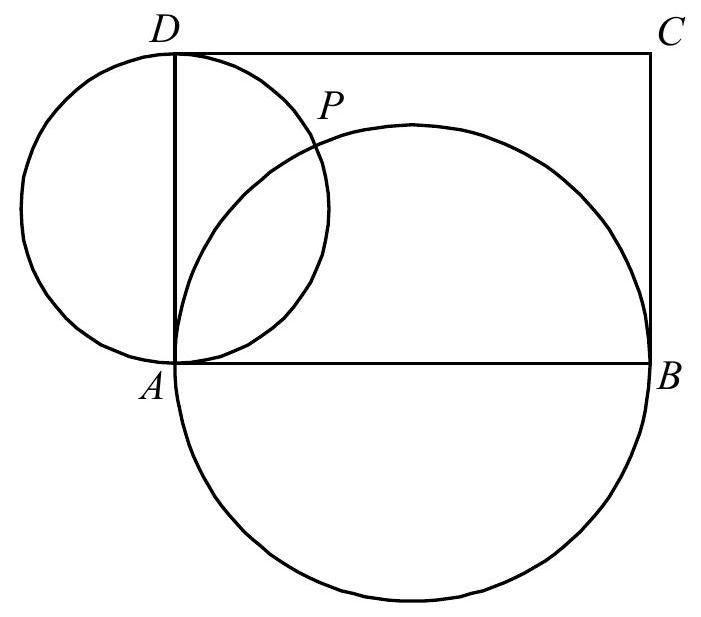
\includegraphics[max width=\textwidth, center]{2024_11_21_603d5c1b2a7d8d68f45fg-14}\\

\includegraphics[max width=\textwidth, center]{2024_11_21_603d5c1b2a7d8d68f45fg-14(1)}

\section*{Zadanie 30. (2 pkt)}
Uzasadnij, że jeśli \(\left(a^{2}+b^{2}\right)\left(c^{2}+d^{2}\right)=(a c+b d)^{2}\), to \(a d=b c\).\\

\includegraphics[max width=\textwidth, center]{2024_11_21_603d5c1b2a7d8d68f45fg-15(1)}

\section*{Zadanie 31. (2 pkt)}
Oblicz, ile jest liczb naturalnych czterocyfrowych, w których zapisie pierwsza cyfra jest parzysta, a pozostałe nieparzyste.\\

\includegraphics[max width=\textwidth, center]{2024_11_21_603d5c1b2a7d8d68f45fg-15}

Odpowiedź:

\section*{Zadanie 32. (4 pkt)}
Ciag \((1, x, y-1)\) jest arytmetyczny, natomiast ciag \((x, y, 12)\) jest geometryczny. Oblicz \(x\) oraz \(y\) i podaj ten ciąg geometryczny.

\begin{center}
\begin{tabular}{|c|c|c|c|c|c|c|c|c|c|c|c|c|c|c|c|c|c|c|c|c|c|c|}
\hline
 &  &  &  &  &  &  &  &  &  &  &  &  &  &  &  &  &  &  &  &  &  &  \\
\hline
 &  &  &  &  &  &  &  &  &  &  &  &  &  &  &  &  &  &  &  &  &  &  \\
\hline
 &  &  &  &  &  &  &  &  &  &  &  &  &  &  &  &  &  &  &  &  &  &  \\
\hline
 &  &  &  &  &  &  &  &  &  &  &  &  &  &  &  &  &  &  &  &  &  &  \\
\hline
 &  &  &  &  &  &  &  &  &  &  &  &  &  &  &  &  &  &  &  &  &  &  \\
\hline
 &  &  &  &  &  &  &  &  &  &  &  &  &  &  &  &  &  &  &  &  &  &  \\
\hline
 &  &  &  &  &  &  &  &  &  &  &  &  &  &  &  &  &  &  &  &  &  &  \\
\hline
 &  &  &  &  &  &  &  &  &  &  &  &  &  &  &  &  &  &  &  &  &  &  \\
\hline
 &  &  &  &  &  &  &  &  &  &  &  &  &  &  &  &  &  &  &  &  &  &  \\
\hline
 &  &  &  &  &  &  &  &  &  &  &  &  &  &  &  &  &  &  &  &  &  &  \\
\hline
 &  &  &  &  &  &  &  &  &  &  &  &  &  &  &  &  &  &  &  &  &  &  \\
\hline
 &  &  &  &  &  &  &  &  &  &  &  &  &  &  &  &  &  &  &  &  &  &  \\
\hline
 &  &  &  &  &  &  &  &  &  &  &  &  &  &  &  &  &  &  &  &  &  &  \\
\hline
 &  &  &  &  &  &  &  &  &  &  &  &  &  &  &  &  &  &  &  &  &  &  \\
\hline
 &  &  &  &  &  &  &  &  &  &  &  &  &  &  &  &  &  &  &  &  &  &  \\
\hline
 &  &  &  &  &  &  &  &  &  &  &  &  &  &  &  &  &  &  &  &  &  &  \\
\hline
 &  &  &  &  &  &  &  &  &  &  &  &  &  &  &  &  &  &  &  &  &  &  \\
\hline
 &  &  &  &  &  &  &  &  &  &  &  &  &  &  &  &  &  &  &  &  &  &  \\
\hline
 &  &  &  &  &  &  &  &  &  &  &  &  &  &  &  &  &  &  &  &  &  &  \\
\hline
 &  &  &  &  &  &  &  &  &  &  &  &  &  &  &  &  &  &  &  &  &  &  \\
\hline
 &  &  &  &  &  &  &  &  &  &  &  &  &  &  &  &  &  &  &  &  &  &  \\
\hline
 &  &  &  &  &  &  &  &  &  &  &  &  &  &  &  &  &  &  &  &  &  &  \\
\hline
 &  &  &  &  &  &  &  &  &  &  &  &  &  &  &  &  &  &  &  &  &  &  \\
\hline
 &  &  &  &  &  &  &  &  &  &  &  &  &  &  &  &  &  &  &  &  &  &  \\
\hline
 &  &  &  &  &  &  &  &  &  &  &  &  &  &  &  &  &  &  &  &  &  &  \\
\hline
 &  &  &  &  &  &  &  &  &  &  &  &  &  &  &  &  &  &  &  &  &  &  \\
\hline
 &  &  &  &  &  &  &  &  &  &  &  &  &  &  &  &  &  &  &  &  &  &  \\
\hline
 &  &  &  &  &  &  &  &  &  &  &  &  &  &  &  &  &  &  &  &  &  &  \\
\hline
 &  &  &  &  &  &  &  &  &  &  &  &  &  &  &  &  &  &  &  &  &  &  \\
\hline
 &  &  &  &  &  &  &  &  &  &  &  &  &  &  &  &  &  &  &  &  &  &  \\
\hline
 &  &  &  &  &  &  &  &  &  &  &  &  &  &  &  &  &  &  &  &  &  &  \\
\hline
 &  &  &  &  &  &  &  &  &  &  &  &  &  &  &  &  &  &  &  &  &  &  \\
\hline
 &  &  &  &  &  &  &  &  &  &  &  &  &  &  &  &  &  &  &  &  &  &  \\
\hline
 &  &  &  &  &  &  &  &  &  &  &  &  &  &  &  &  &  &  &  &  &  &  \\
\hline
 &  &  &  &  &  &  &  &  &  &  &  &  &  &  &  &  &  &  &  &  &  &  \\
\hline
 &  &  &  &  &  &  &  &  &  &  &  &  &  &  &  &  &  &  &  &  &  &  \\
\hline
 &  &  &  &  &  &  &  &  &  &  &  &  &  &  &  &  &  &  &  &  &  &  \\
\hline
 &  &  &  &  &  &  &  &  &  &  &  &  &  &  &  &  &  &  &  &  &  &  \\
\hline
 &  &  &  &  &  &  &  &  &  &  &  &  &  &  &  &  &  &  &  &  &  &  \\
\hline
 &  &  &  &  &  &  &  &  &  &  &  &  &  &  &  &  &  &  &  &  &  &  \\
\hline
 &  &  &  &  &  &  &  &  &  &  &  &  &  &  &  &  &  &  &  &  &  &  \\
\hline
 &  &  &  &  &  &  &  &  &  &  &  &  &  &  &  &  &  &  &  &  &  &  \\
\hline
 &  &  &  &  &  &  &  &  &  &  &  &  &  &  &  &  &  &  &  &  &  &  \\
\hline
\end{tabular}
\end{center}

Odpowiedź:

\section*{Zadanie 33. (4 pkt)}
Punkty \(A=(1,5), B=(14,31), C=(4,31)\) są wierzchołkami trójkąta. Prosta zawierająca wysokość tego trójkąta poprowadzona z wierzchołka \(C\) przecina prostą \(A B\) w punkcie \(D\). Oblicz długość odcinka \(B D\).\\

\includegraphics[max width=\textwidth, center]{2024_11_21_603d5c1b2a7d8d68f45fg-17}

Odpowiedź:

\section*{Zadanie 34. (5 pkt)}
Droga z miasta A do miasta B ma długość 474 km . Samochód jadacy z miasta A do miasta B wyrusza godzinę później niż samochód z miasta B do miasta A. Samochody te spotykają się w odległości 300 km od miasta B. Średnia prędkość samochodu, który wyjechał z miasta A, liczona od chwili wyjazdu z A do momentu spotkania, była o \(17 \mathrm{~km} / \mathrm{h}\) mniejsza od średniej prędkości drugiego samochodu liczonej od chwili wyjazdu z B do chwili spotkania. Oblicz średnią prędkość każdego samochodu do chwili spotkania.\\

\includegraphics[max width=\textwidth, center]{2024_11_21_603d5c1b2a7d8d68f45fg-18}

Odpowiedź:\\

\includegraphics[max width=\textwidth, center]{2024_11_21_603d5c1b2a7d8d68f45fg-19}


\end{document}